Wie Abbildung \ref{Versuchsaufbau} zeigt, bestand der Versuchsaufbau im Wesentlichen aus einem Gestell, in das Metallstäbe verschiedener Querschnittsflächen sowohl einseitig, als auch zweiseitig eingespannt werden konnten. \\
Zunächst wurden die verwendeten Stäbe, ein runder und ein eckiger, in Länge und Durchmesser vermessen und gewogen. \\
Danach wurden die Stäbe einzeln und einseitige in die Vorrichtung eingespannt und bei verschiedenen Abständen $x$ zur Einspannung wurde die Auslenkung $D(x)$ je einmal mit einem Gewicht am Ende der Stange und einmal ohne gemessen. \\
Zuletzt wurde der eckige Stab beidseitig eingespannt und ein Gewicht in der Mitte eingehängt. Hier wurde die Auslenkung $D$ bei verschiedenen Abständen zum (näherliegenden) Rand je links und rechts des Gewichts gemessen.
\begin{figure}[ht!]
	\centering
	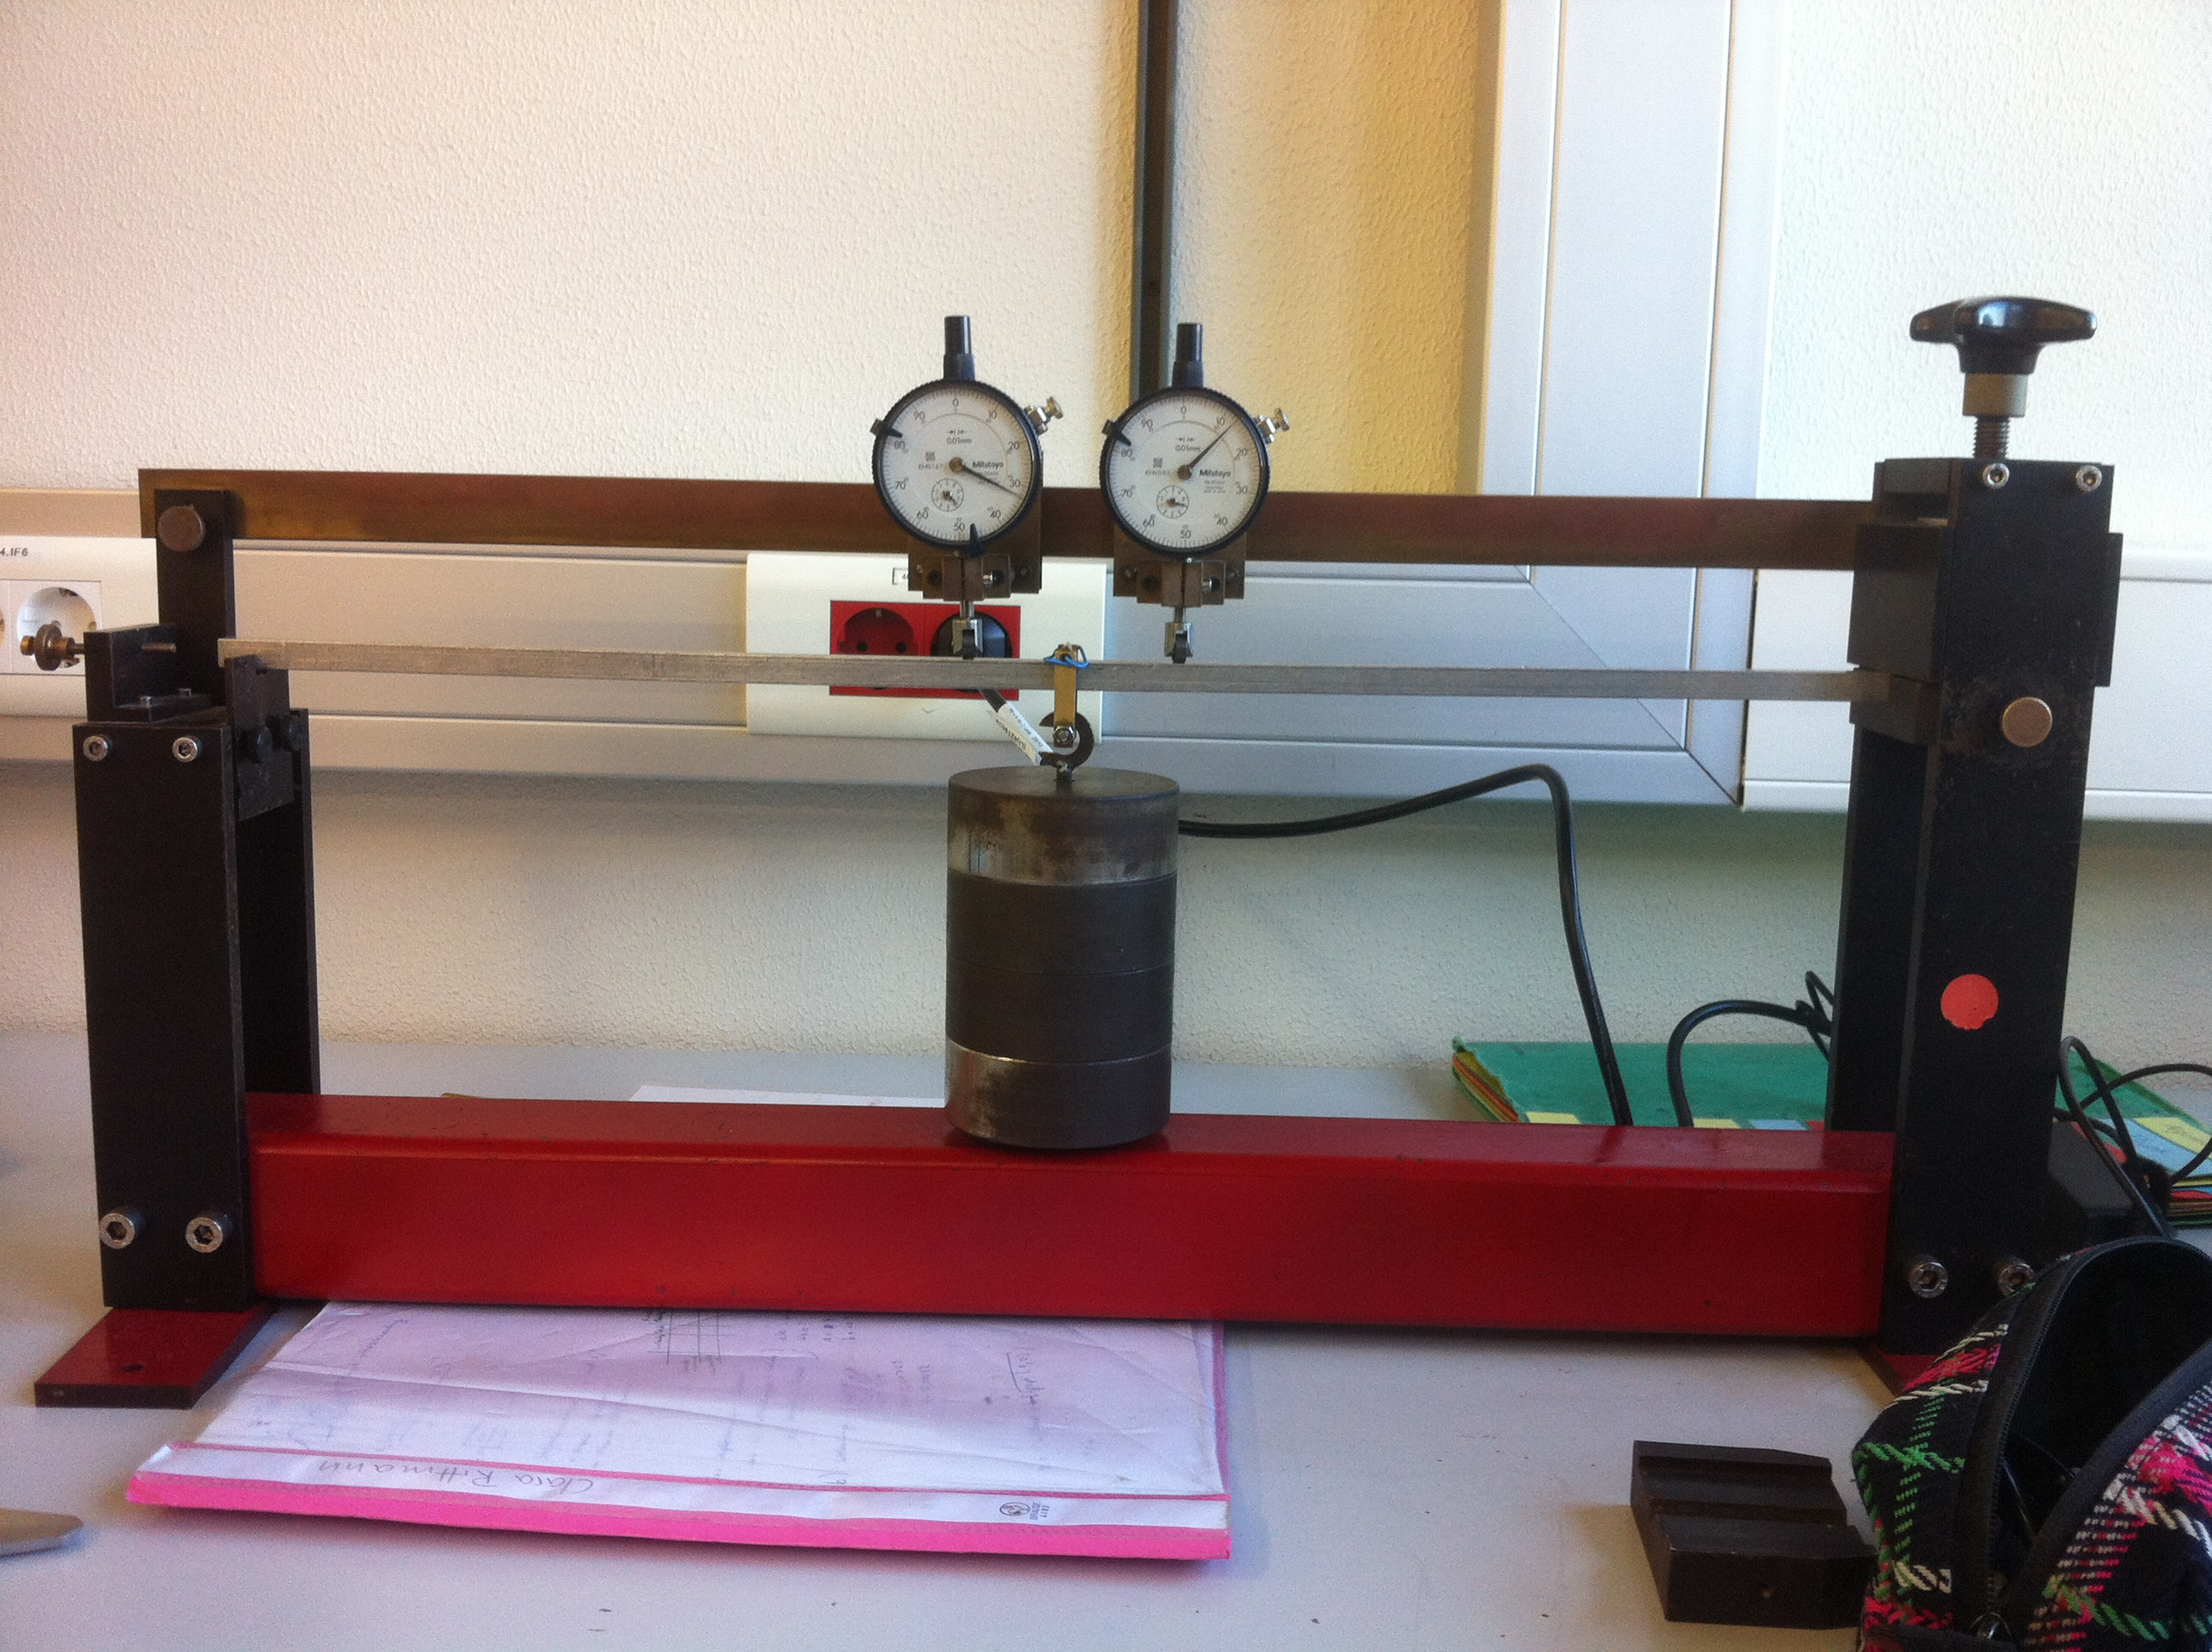
\includegraphics[width=0.8\textwidth]{Versuchsaufbau.JPG}
	\caption{Versuchsaufbau mit beidseitig eingespanntem Stab}
	\label{Versuchsaufbau}
\end{figure}